\lecture{20}{7. November 2024}{gravitation – fortsat}
\section{Keplers Love}
Kepler opstillede 3 love for planeters bevægelser.

\begin{sæt}[Keplers love]
  \begin{itemize}
    \item Planeterne beskriver elliptiske baner med solen i det ene brændpunkt.
    \item Radiusvektor fra solen til planeten overstryger et konstant areal pr. tidsenhed.
    \item Forholdet mellem kvadratet på en planets omløbstid i dens bane om solen og trejde potens af dens halve storakse er ens for alle planeter.
      \[ 
        T = \frac{2\pi r}{v} = 2\pi r \cdot \sqrt{\frac{r}{Gm_E}} = \frac{2\pi r^{\frac{3}{2}}}{\sqrt{Gm_E}}
      .\]
\end{itemize}
\tcblower
\textbf{Bevis af Keplers 2. lov}
Arealet, $\mathrm{d}a$, som en planet overstryger over en lille tidsperiode $\, \mathrm{d}t$ er en trekant. Denne må altså kunne beskrives som
\[ 
\, \mathrm{d}A = \frac{1}{2}r\cdot r \cdot \, \mathrm{d}\theta
.\]
Og hvis vi dividerer med tiden $\, \mathrm{d}t$ fås
\begin{align*}
  \frac{\mathrm{d}A}{\mathrm{d}t} &= \frac{1}{2} r \cdot r \cdot \frac{\mathrm{d}\theta}{\mathrm{d}t} \\
  &= \frac{1}{2}r(r\omega) \\
  &= \frac{1}{2}rv_t \\
  &= \frac{1}{2}r(|\Vec{v}| \sin\phi) \\
  &= \frac{1}{2} \left| \Vec{r} \times \Vec{v} \right| \\
  &= \frac{1}{2m} \left| \Vec{r}\times(m \Vec{v}) \right| \\
  &= \frac{1}{2m} \left| \Vec{r} \times \Vec{\rho} \right|
.\end{align*}
Hvis $\frac{\mathrm{d}A}{\mathrm{d}t} = \mathrm{const.}$ så er $\Vec{r} \times \Vec{\rho} = \mathrm{const.}$. Fra før har vi
\[ 
  \frac{\mathrm{d}A}{\mathrm{d}t} = \frac{1}{2m} \left| \Vec{r} \times \Vec{\rho} \right| = \frac{1}{2m} L
,\]
hvor $L$ er impulsmomentet. Derudover ved vi at den tidsafledede af impulsmomentet er 
\[ 
\frac{\mathrm{d}L}{\mathrm{d}t} = \tau = \Vec{r} \times \Vec{F}
.\]
Og idet $\Vec{r} \times \Vec{F} = 0$ så er
\[ 
\frac{\mathrm{d}L}{\mathrm{d}t} = 0
.\]
\end{sæt}

\section{Massedistirbution af sfæriske opbjekter}
Vi kan for jævntfordelte sfæriske objekter ``lade som om'' at al massen er koncentreret i centrum.

\begin{figure} [ht]
  \centering
  \caption{Diagram af kugleskal}
  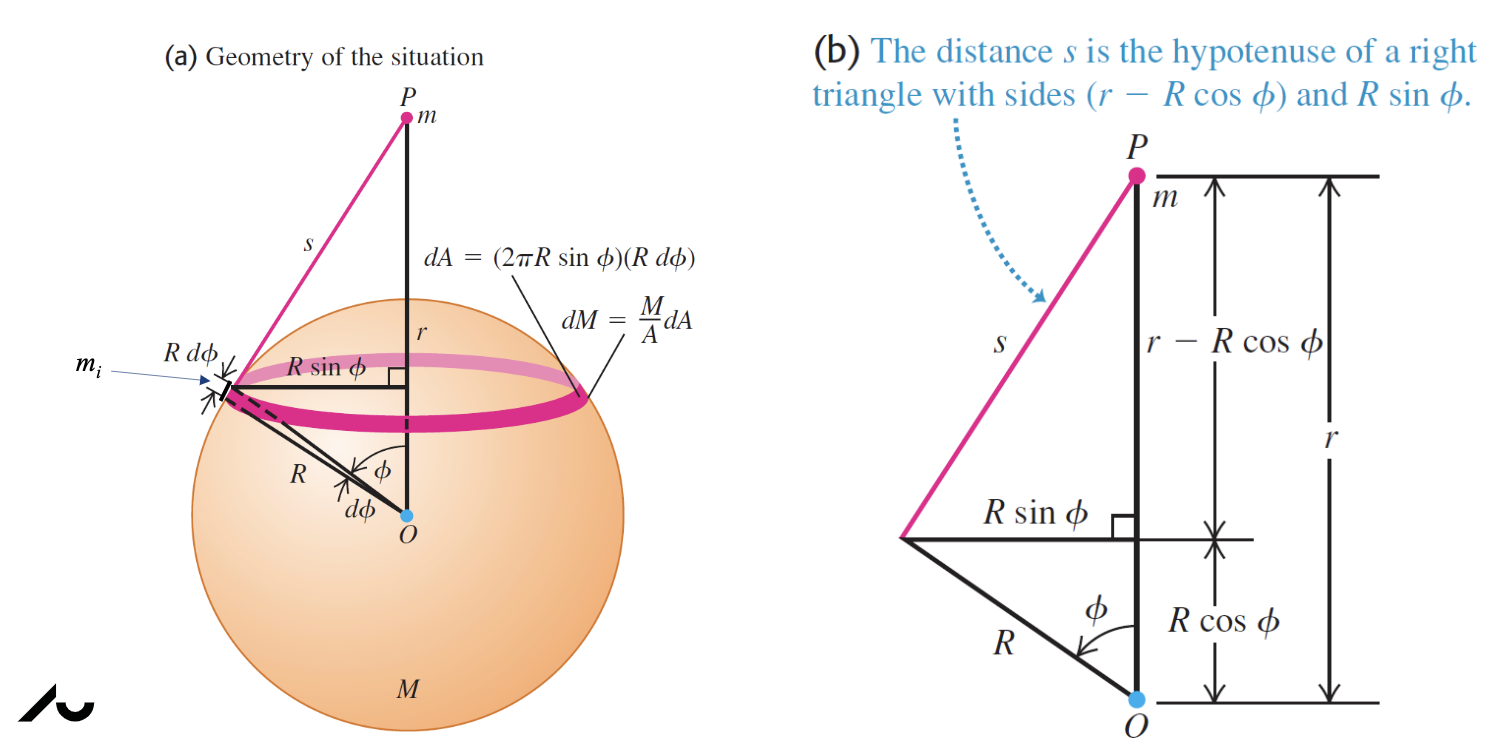
\includegraphics[width=0.7\linewidth]{./figures/F20_1.png}
  \label{fig:F20_1}
\end{figure}

\begin{sæt}[Massemidtpunktet af en jævntfordelt hul skal er i dets centrum]
  En simplificering af sætningen ovenfor er for tilfældet af med en hul skal. Dette vil herunder eftervises.
  \tcblower
  For et element på skallen, $m_i$ har vi at det gravitationelle potentiale for elementet er
  \[ 
  U_i = - \frac{Gm_im}{S}
  .\]
  Dette kan vi summere op for en ``ring'' om cirklen (tænk stykket mellem to bredde/længdegrader). For én ring har vi
  \[ 
    \mathrm{d}U = - \sum_{i} \frac{Gmm_i}{S} = - \frac{Gm}{S} \, \mathrm{d}M 
  ,\]
  Hvor
  \[ 
  \, \mathrm{d}M = \sum_{i} m_i
  .\]
  Vi får altså at
  \[ 
    \frac{\mathrm{d}M}{M} = \frac{\mathrm{d}A}{A} \implies \, \mathrm{d}M = M \frac{\mathrm{d}A}{A}
  .\]
  Arealet af ringen $\mathrm{d}A$ er
  \[ 
  \mathrm{d}A = 2\pi\cdot (R\cdot \sin\phi)R \, \mathrm{d}\phi
  .\]
  Hvor $\, \mathrm{d}\phi$ er den lille vinkelændring mellem toppen og bunden eller den ene og den anden kant af dit ``bredde- eller længdegradsbånd''. Bemærk at i ovenstående er $\mathrm{omkredsen} = 2\pi(R \sin\phi)$ og $\mathrm{bredden} = R \, \mathrm{d}\phi$. Vi omskriver til
  \[ 
  \mathrm{d}A = 2\pi R^2 \sin\phi \, \mathrm{d}\phi
  .\]
  Overfladearealet af en kugle er kendt til at være
  \[ 
  A = 4\pi R^2
  .\]
  Vi har altså at
  \[ 
  \mathrm{d}M = M \frac{\mathrm{d}A}{A} = \frac{1}{2}M \sin\phi \, \mathrm{d}\phi
  .\]
  Så vi får
  \[ 
  \mathrm{d}U = - \frac{Gm}{S}\frac{1}{2}M \sin\phi \, \mathrm{d}\phi
  .\]
  Vi vælger at isolere for $s$ istedet for for $\phi$. Altså findes fra \autoref{fig:F20_1} at
  \[ 
  S^2 = (R \sin\phi)^2 + (r-R \cos\phi)^2 = R^2 \sin^2\phi + r^2 + R^2 \cos^2 \phi - 2rR \cos\phi
  .\]
  Dette omskrives til
  \[ 
  S^2 = R^2 + r^2 - 2rR \cos\phi
  .\]
  Vi differentierer med hensyn til $S$, idet $\phi$ er en funktion af $S$. Vi får at
  \[ 
  \frac{\mathrm{d}}{\mathrm{d}s}(-\cos\phi(s)) = \frac{\mathrm{d}}{\mathrm{d}\phi}(-\cos\phi) \frac{\mathrm{d}\phi}{\mathrm{d}s}   
  .\]
  Altså har vi
  \begin{align*}
    2S &= 2rR \sin\phi \frac{\mathrm{d}\phi}{\mathrm{d}s} \\
    S \, \mathrm{d}S &= rR \sin\phi \, \mathrm{d}\phi \\
    \sin \phi \, \mathrm{d}\phi = \frac{S \, \mathrm{d}S}{rR}
  .\end{align*}
  Vi sætter ind i udtrykket for $\mathrm{d}U$ så
  \begin{align*}
    \mathrm{d}U &= -\frac{1}{2}\frac{Gm}{s}M \sin\phi \, \mathrm{d}\phi \\
    &= -\frac{1}{2}\frac{Gm}{S}MS \, \mathrm{d}S \frac{1}{rR}\\
    &= -\frac{1}{2rR} GmM \, \mathrm{d}S \\
  .\end{align*}
  Vi integrerer over $S$ så vi får hele potentialet. For startpunktet $\phi = 0$ har vi $S = r-R$ og for slutpunktet $\phi = \pi$ har vi $S = r+R$. Vi har altså
  \begin{align*}
    U &= - \frac{1}{2rR}GMm \int_{r-R}^{r+R} \, \mathrm{d}s \\
    &= -\frac{1}{2rR}GmM \left\{ r+R - (r-R) \right\} \\
    &= -\frac{1}{r}GmM
  .\end{align*} 
  Dette er den potentielle energi mellem to punktmasser. Altså er det vist at massemidtpunktet er uafhængigt af den store radius $R$ og at midten derfor ikke flytter sig selvom den store radius $R$ stiger. Bemærk i øvrigt, at hvis massen var placeret inde i skallen istedet for på skallen får vi i stedet
  \begin{align*}
    U &= - \frac{1}{2rR}GMm \int_{R-r}^{R+r} \, \mathrm{d}S \\
      &= - \frac{GMm}{2Rr} \left\{ (R+r) - (R-r) \right\} \\
      &= - \frac{GMm}{R}
  .\end{align*}
  Dette afhænger ikke af $r$ og derfor må det gælde at uanset placering vil en prøvemasse inde i skallen have konstant potentiale. 
\end{sæt}
Bemærk at det ovenstående også betyder at $W_g = 0 \implies F_g = 0$. Der er derfor heller ikke et tyngdefelt inde i skallen. Dette betyder også at Jules Vernes ``en rejse til jordens indre'' er dybt urealistisk. Derfor er der også en simplificering af problemet, hvor en mand hopper gennem en tunnel gennem jorden idet han til enhver tid kun vil opleve en gravitationskraft fra den kugle af jorden der går fra jordens centrum og ud til ham. 
